Some programming languages allow specification of default values directly in the method signature.
In this case, if the caller does not specify the value of the parameter, the default value is used.
This feature is often combined with named parameters.
Another approach is to specify optional parameters at the end of the parameter list.

Figure~\ref{fig:def_specification_of_default_values} shows example with specified default values in the interface
method signature.
For demonstration purposes, 2 new parameters have been added: \textit{packetLogger} used for logging serialized
packets and \textit{addressResolver} used for resolution of named addresses into IP address representation.
In this example, default values are assigned to the \textit{maxResponseTime}, \textit{packetLogger},
and \textit{addressResolver} parameters.

\begin{figure}[!htb]
    \centering
    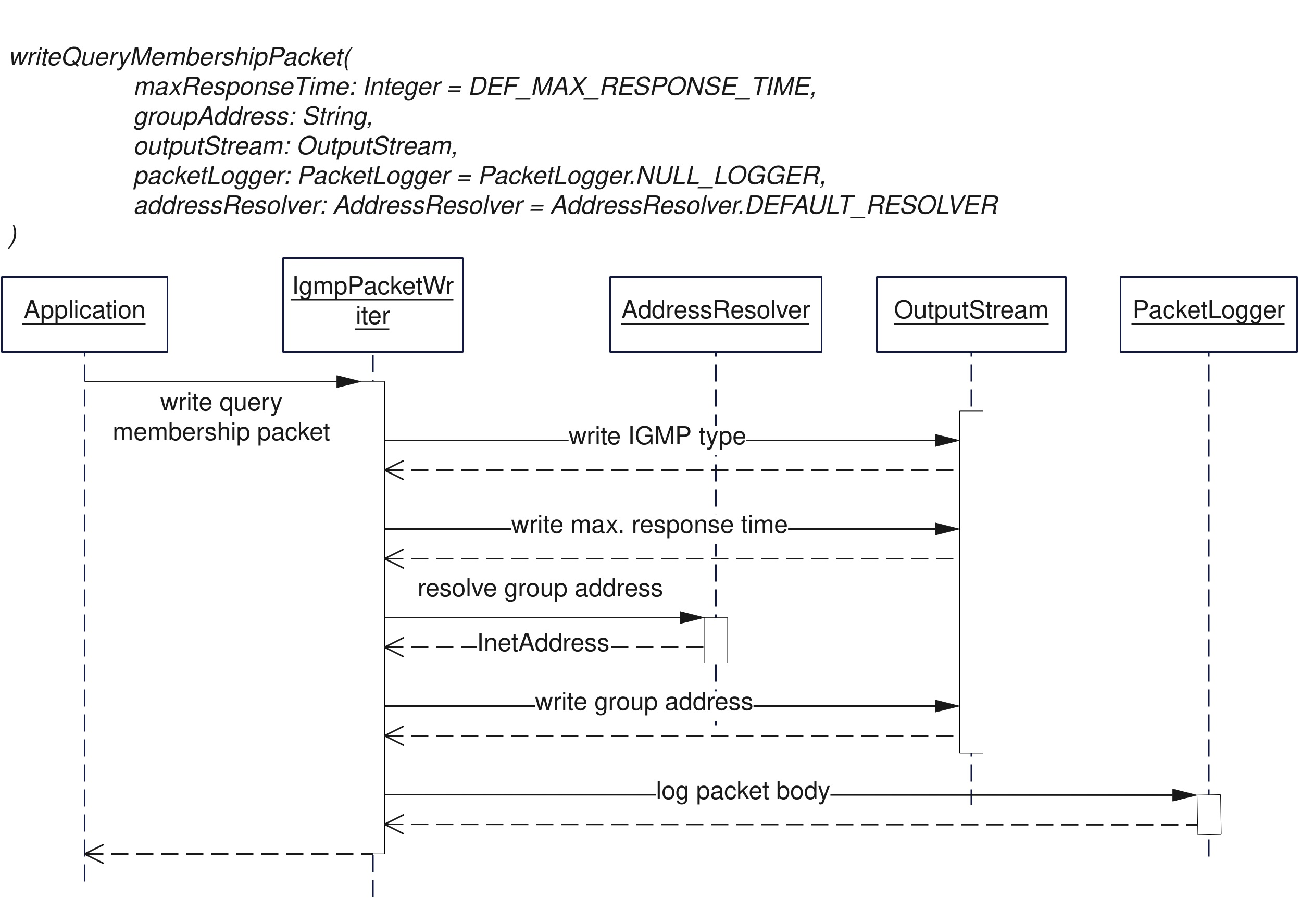
\includegraphics[width=1.0
    \textwidth]{def_specification_of_default_values}
    \caption{Default Values: Specification of default values}
    \label{fig:def_specification_of_default_values}
\end{figure}

\begin{itemize}
    \item \textit{maxResponseTime}: It has a primitive \textit{Integer} type.
    In this case, it is possible to directly specify the default value without creation of additional entities.
    \item \textit{packetLogger}: This parameter has PacketLogger type which is the next interface.
    The default value is set to \textit{PacketLogger.NULL\_LOGGER} constant which follows Null Object design pattern.
    Figure~\ref{fig:def_null_logger} demonstrates the implementation of this constant.
    \textit{NULL\_LOGGER} is the instance of the PacketLogger subclass \textit{NullPacketLogger} that does
    not log anything, just ignores all input calls.
    If the API did not use Null Object design pattern, it would be necessary to handle the null reference in the
    implementation of the \textit{writeQueryMembershipPacket} method.
    \item \textit{addressResolver}: The parameter is of type AddressResolver that is described by distinct interface.
    The default value is set to \textit{AddressResolver.DEFAULT\_RESOLVER} constant which represents instance of dummy
    implementation of the \textit{AddressResolver} interface.
    It does not try to resolve the address and only returns the input address,
    if it matches the pattern of the IP address.
    Figure~\ref{fig:def_default_address_resolver} shows the implementation of the constant in detail.
    It is more complex than the Null Object design pattern since implementation contains at least
    simple pattern-matching logic.
\end{itemize}

\begin{figure}[!htb]
    \centering
    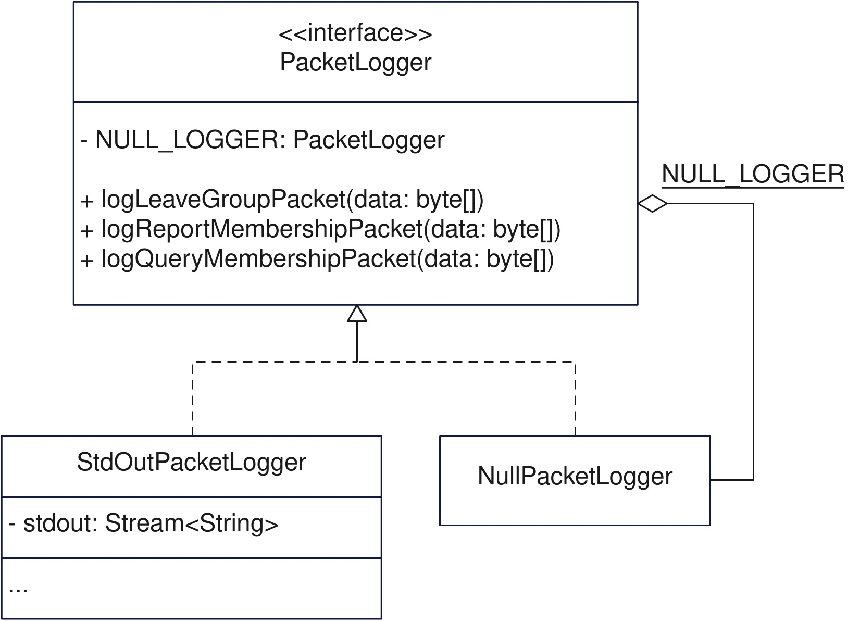
\includegraphics[width=0.66
    \textwidth]{def_null_logger}
    \caption{Default Values: Null logger}
    \label{fig:def_null_logger}
\end{figure}

\begin{figure}[!htb]
    \centering
    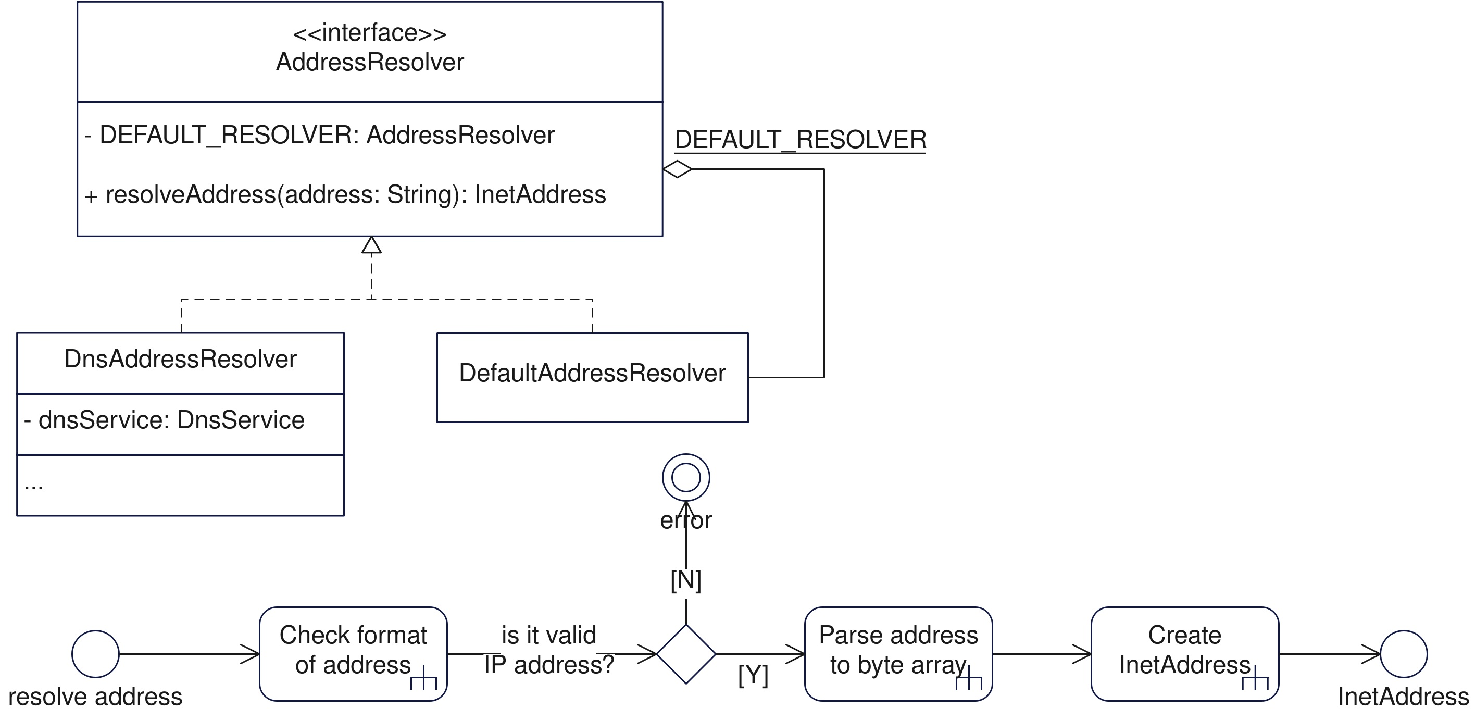
\includegraphics[width=1.0
    \textwidth]{def_default_address_resolver}
    \caption{Default Values: Default address resolver}
    \label{fig:def_default_address_resolver}
\end{figure}

Benefits of the Default Values approach:

\begin{itemize}
    \item Improved readability of the method signature - it is clear which parameters are optional and what values
    are used if these parameters are not specified by caller.
    Definition of the method itself is used as a documentation.
    \item Removed handling of null references or values in the implementation of the interface method
    (based on separation of concerns principle).
    It usually consists of repetitive conditional statements that check whether the parameter is null or not.
    Code is more readable and easier to maintain.
\end{itemize}

Drawbacks of the Default Values approach:

\begin{itemize}
    \item Limited flexibility - Default values are static and cannot be changed at runtime.
    This can limit the flexibility of your code, especially if you need to change these values based on certain
    conditions or configurations.
    \item For some complex types it is not always feasible to create a default implementation.
    If type defines method that returns value of some type, it is also necessary to mock return type.
    Also in some languages it is possible to mark a type or method as final, so it is not possible to create
    a subclass from it or override implementation of specific method.
    If type is defined in the external library, we cannot easily update its constraints.
\end{itemize}

Common use-cases of the Default Values approach:

\begin{itemize}
    \item Specification of default values for optional parameters that are not used frequently by clients
    deployed in production environment.
    These parameters can be used, for example, in the debugging mode or in the testing environment.
    \item Avoiding extensive overloading of the method signature - decreasing impact of API Rooting issue.
    If there are many optional parameters, it would be unpractical to create all possible combinations of methods.
    Additional interface methods increase maintenance cost.
\end{itemize}
